\documentclass[12pt,compress,ngerman,utf8,t,usenames,dvipsnames]{beamer}
\usepackage{etex}
\usepackage[ngerman]{babel}
\usepackage{graphicx}
\usepackage[export]{adjustbox}
\usepackage{multicol}
% \usepackage{animate}
% \usepackage{media9}


\usetheme[numbering=fraction, progressbar=frametitle]{metropolis}


\date{\today}
\institute{University of Freiburg}
\titlegraphic{\vspace{4cm} \hspace{9cm} 
\includegraphics[height=2cm]{template/Logo-Uni-Freiburg.png}}
\graphicspath{ {./template/} {./bioinfII/} {./bioinfII/images/} }

\title{A Simple Protocol for the Inference of RNA Global Pairwise Alignments}
\author{Felix Karg}

\newif\ifonline
\onlinefalse
% \onlinefalse

\AtBeginSection[]
{
    \large
    \begin{frame}{Content}
%         \begin{multicols}{2}
            \tableofcontents[currentsection]
%         \end{multicols}
        \clearpage
    \end{frame}
}

\AtBeginSubsection[]
{
    \large
    \begin{frame}{Content}
%         \begin{multicols}{2}
            \tableofcontents[currentsection,currentsubsection]
%         \end{multicols}
        \clearpage
    \end{frame}
}

% \vspace{0.1cm}



\newcommand{\code}[1]{
    \begin{center}
    \setlength{\fboxrule}{1pt}
    \setlength{\fboxsep}{8pt}
        {\fbox{\parbox{0.81\textwidth}{#1}}}
   \end{center}
}




\begin{document}

\maketitle

% multicols from:
% https://tex.stackexchange.com/questions/24343/splitting-toc-into-two-columns-on-single-frame-in-beamer

%%%%%%%%%%%%%%%%%%%%%%%%%%%%%%%%%%%%%%%%%%%%%%%%%%%%%%%%%%%%%%%%%%%%%%%%%%%%%%%%%%%%%%%%%%%%%%%%%%%%%%%%%%%%%%%%%%%

\begin{frame}{Content}
    \large
%     \begin{multicols}{2}
%        \tableofcontents[hidesubsections]
        \tableofcontents[]
%     \end{multicols}
    % \clearpage
\end{frame}


% Topics:
%
% Recap: Sequence Similarity / Identity (short: needleman)
% Somewhat: Tree-based alignment
% In-Depth: Sankoff Algorithm (LocARNA)


%%%%%%%%%%%%%%%%%%%%%%%%%%%%%%%%%%%%%%%%%%%%%%%%%%BEGINNING%%%%%%%%%%%%%%%%%%%%%%%%%%%%%%%%%%%%%%%%%%%%%%%%%%%%%%%%
% \section{Recap}



\begin{frame}[c]{}
    \center
    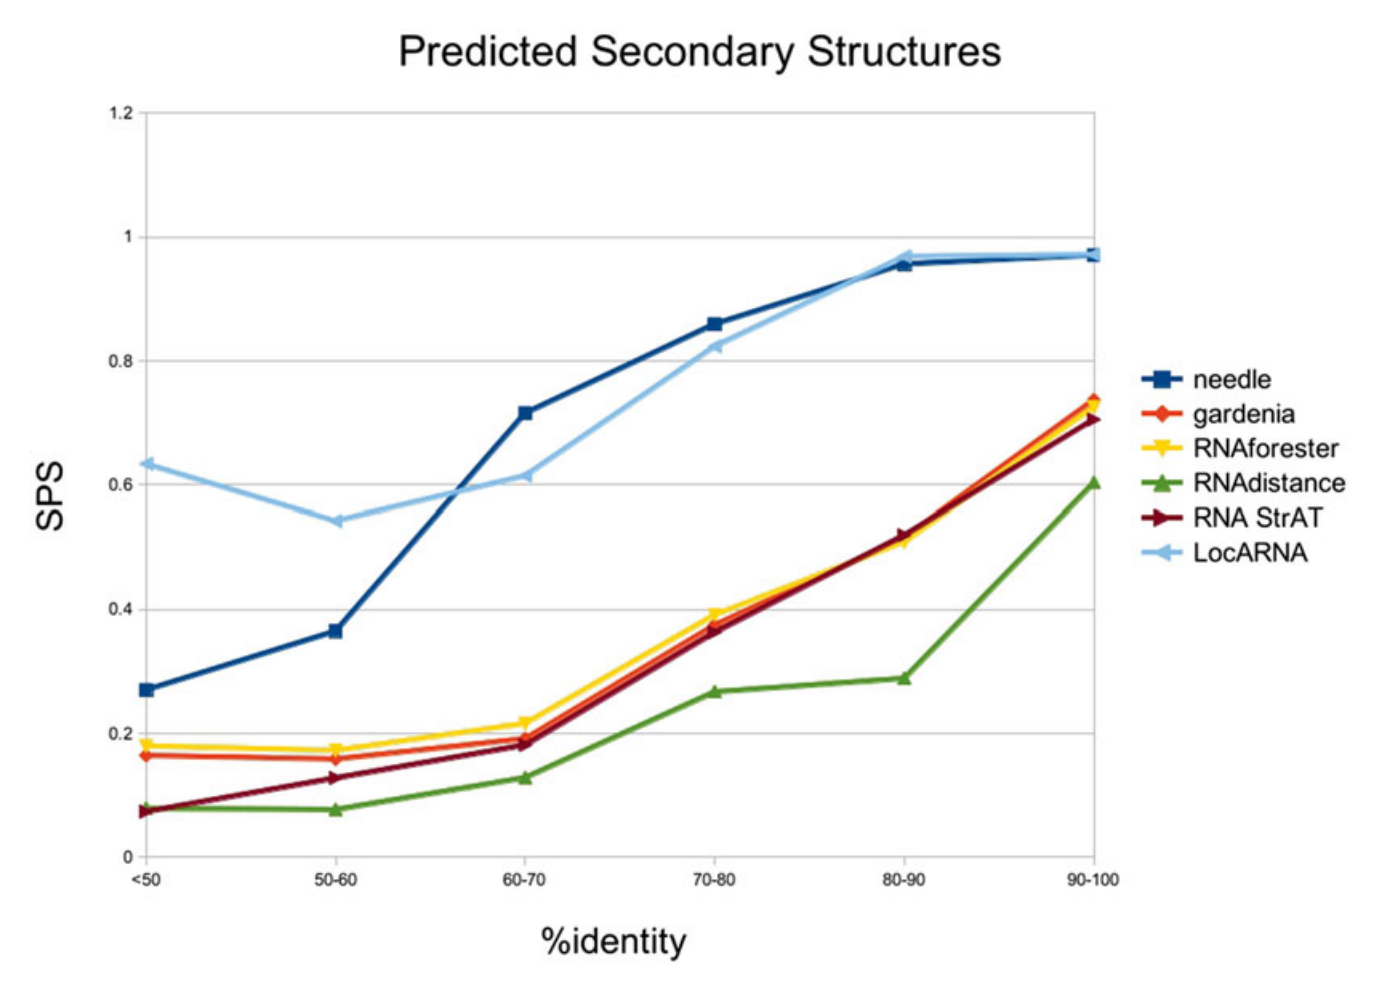
\includegraphics[width=\textwidth]{predicted}
\end{frame}


\begin{frame}[c]{}
    \center
    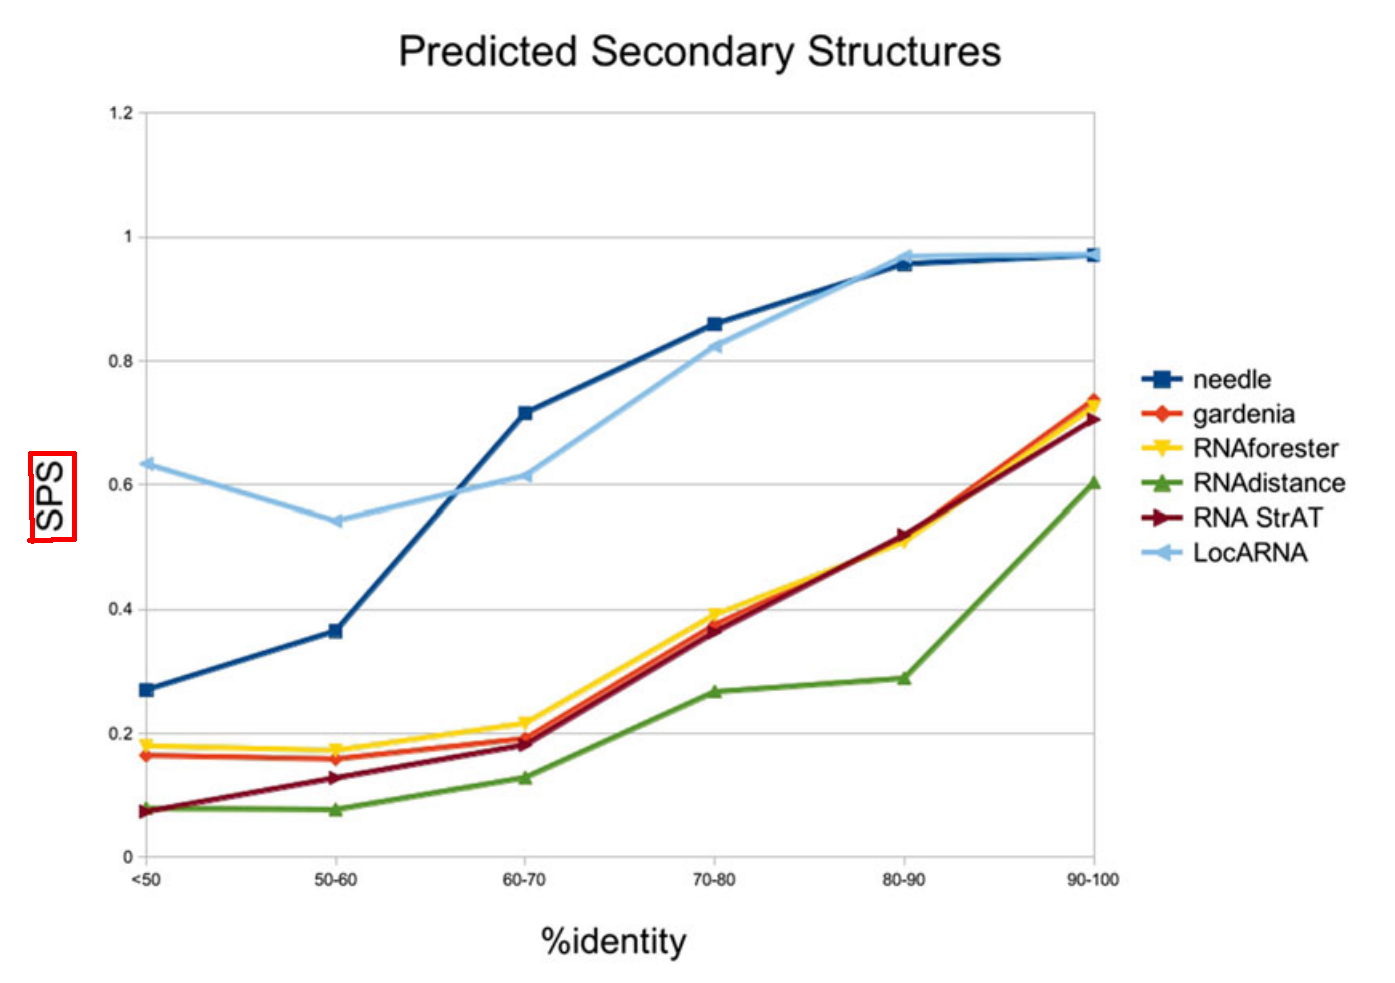
\includegraphics[width=\textwidth]{predicted_sps}
\end{frame}


\begin{frame}[c]{SPS - introduction}
    Sum of Pairs Score
    \newline
%    \vspace{2cm}
    \newline
    \pause
    Used to measure the \only<2-2>{alignment}\only<3->{similiarity} of two RNA sequences
\end{frame}


\begin{frame}[c]{Sequence Similiarity - Example}
    A: \only<4-5>{AAGGC}\only<1-1>{AAGGC}\only<2-3>{{\color{ForestGreen} AAGGC}}\only<1,4->{TT}\only<2-3>{{\color{red}TT}} \\
    B: \only<1-1>{AAGGC}\only<2-5>{{\color{ForestGreen} AAGGC}} \\
    C: \only<1-3>{AAGGC}\only<4->{{\color{ForestGreen} AAGGC}}\only<4-5>{{\color{red}AT}}\only<-3>{AT} \newline
    \newline
    Similiarity: \only<3,5>{60\% = 1 - (2 / 5) } \\
    1 - (edit distance / unaligned length of shorter sequence)
\end{frame}


\begin{frame}[c]{Sequence Similiarity - Example}
    A: {\color{ForestGreen}AAGGC}{\color{red}T}{\color{ForestGreen}T} \\
    B: AAGGC \\
    C: {\color{ForestGreen}AAGGC}{\color{red}A}{\color{ForestGreen}T} \newline
    \newline
    Similiarity: \only<2>{ 86\% = 1 - (1 / 7) } \\
    1 - (edit distance / unaligned length of shorter sequence)
\end{frame}


\begin{frame}[c]{}
    \center
    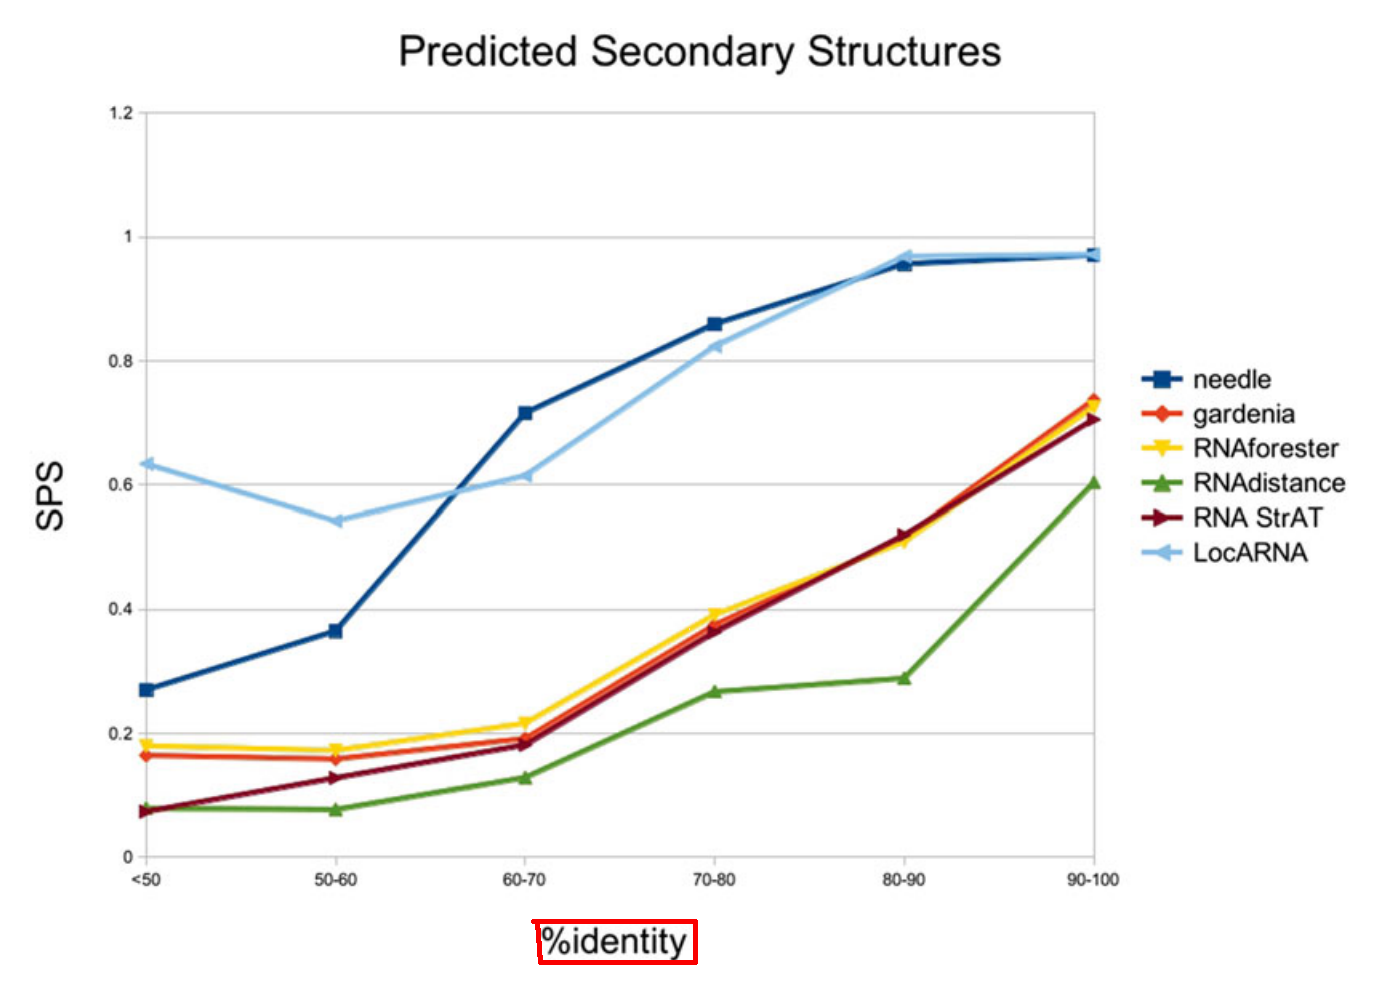
\includegraphics[width=\textwidth]{predicted_identity}
\end{frame}


\begin{frame}[c]{Sequence Identity - Example}
    A: \only<4-5>{AAGGC}\only<1-1>{AAGGC}\only<2-3>{{\color{ForestGreen} AAGGC}}TT \\
    B: \only<1-1>{AAGGC}\only<2-5>{{\color{ForestGreen} AAGGC}} \\
    C: \only<1-3>{AAGGC}\only<4-5>{{\color{ForestGreen} AAGGC}}AT \newline
    \newline
    Identity: \only<3,5>{100\%} \\
    Identical nucleotides / shorter sequence length
\end{frame}


\begin{frame}[c]{Sequence Identity - Example}
    A: {\color{ForestGreen}AAGGC}{\color{red}T}{\color{ForestGreen}T} \\
    B: AAGGC \\
    C: {\color{ForestGreen}AAGGC}{\color{red}A}{\color{ForestGreen}T} \newline
    \newline
    Identity: \only<2>{85\% = 6 / 7} \\
    Identical nucleotides / shorter sequence length
\end{frame}


\begin{frame}[c]{needle}
    \center
    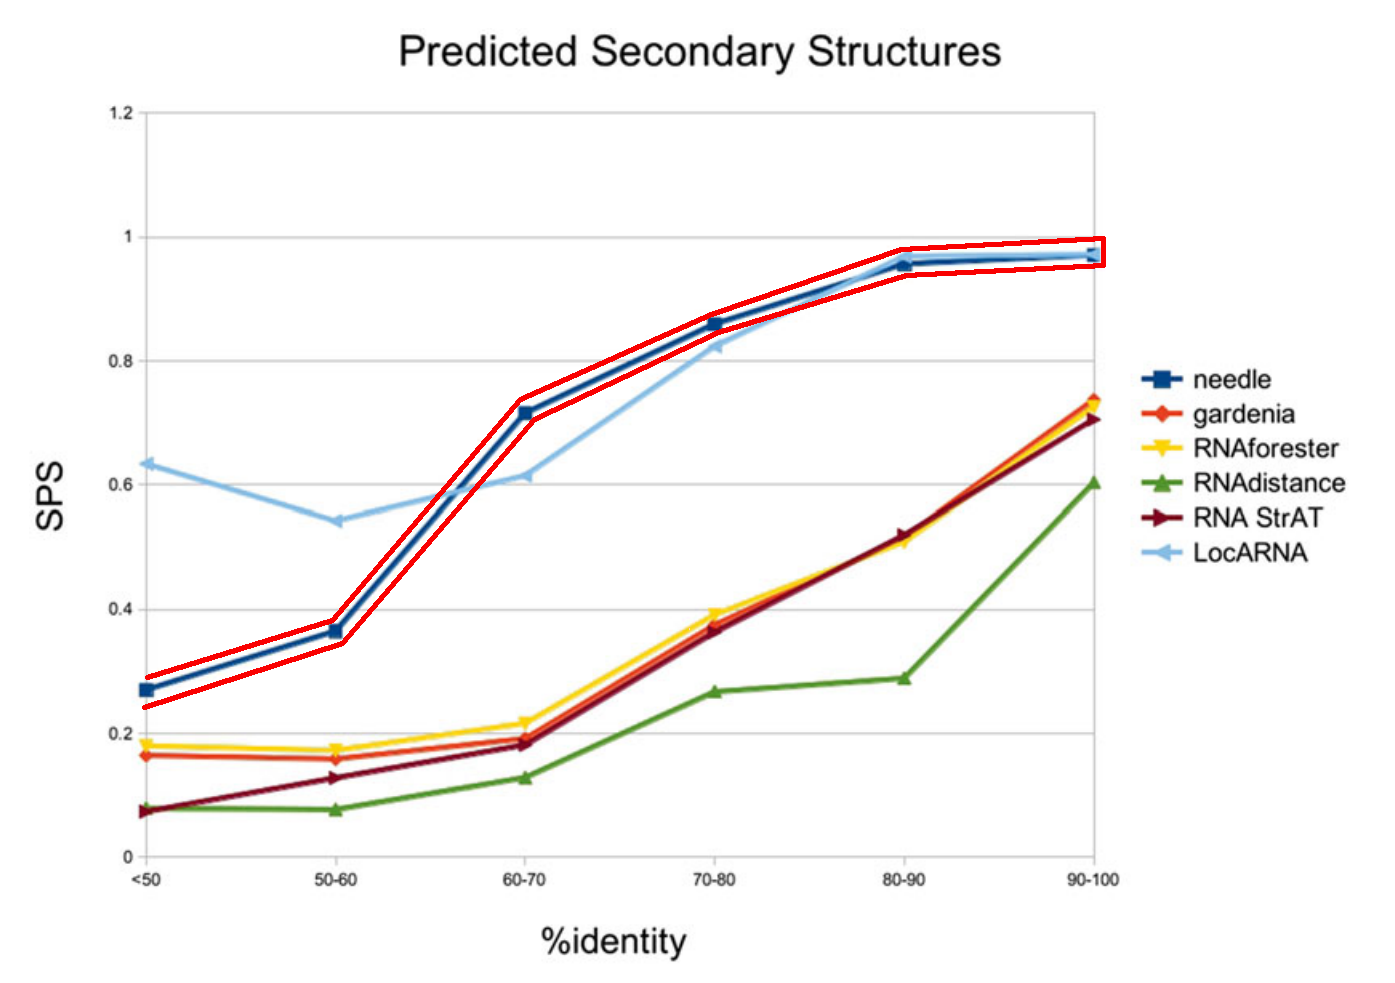
\includegraphics[width=\textwidth]{predicted_needle}
\end{frame}

\begin{frame}[c]{Needleman-Wunsch-Algorithm}
    \center
    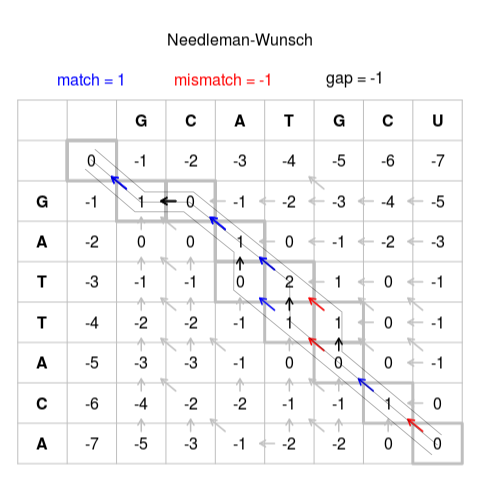
\includegraphics[width=0.75\textwidth]{Needleman-Wunsch_pairwise_sequence_alignment}
\end{frame}












% \section{Tree-Based}


\begin{frame}[c]{Tree-based}
    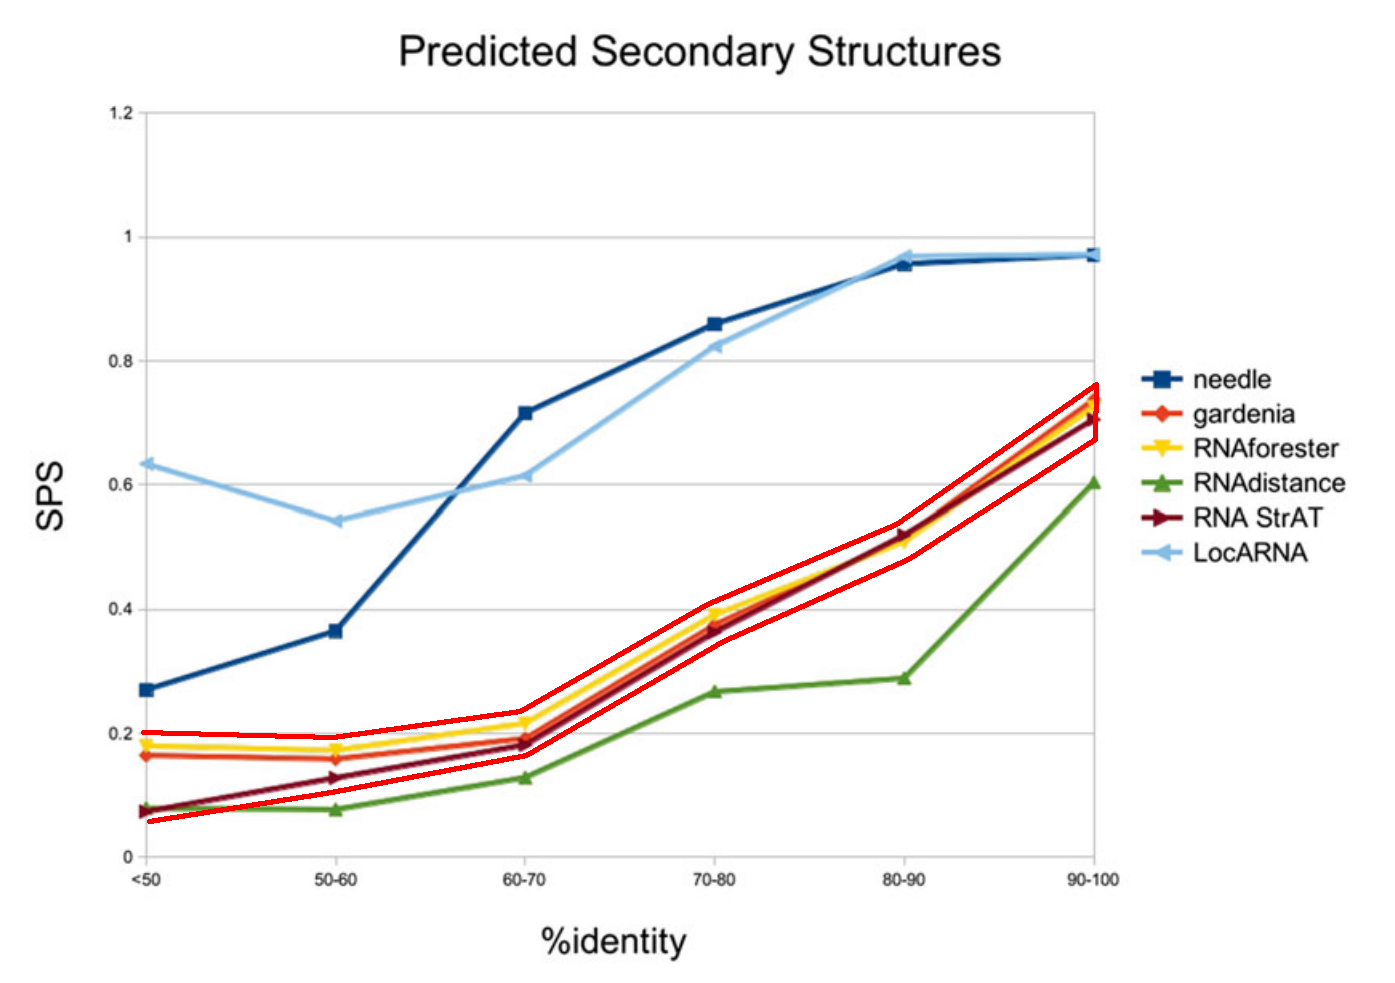
\includegraphics[width=\textwidth]{predicted_tree}
\end{frame}


\begin{frame}[c]{Tree-based}
    \Large
    Using the secondary structure:
    \newline
    \newline
    % trim = l b r t
    \begin{overprint}
    \only<2>{\centering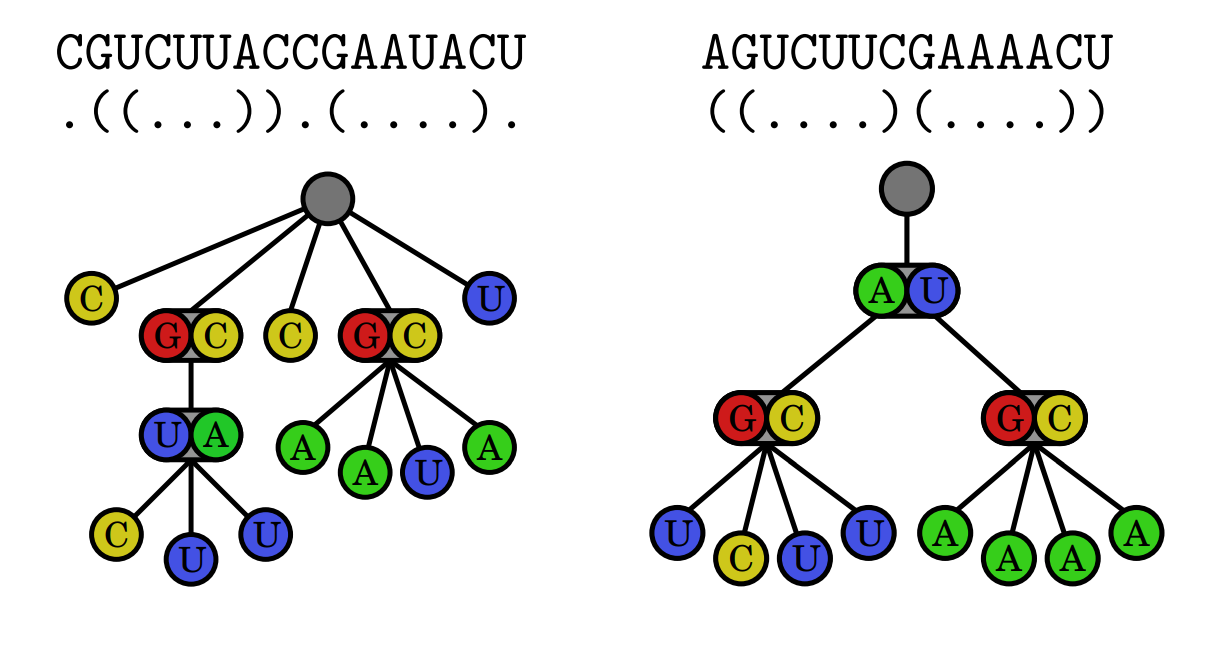
\includegraphics[width=0.47\textwidth, clip=true, trim = 0mm 0mm 230mm 0mm]{tree_sequences}}
    \only<3>{\centering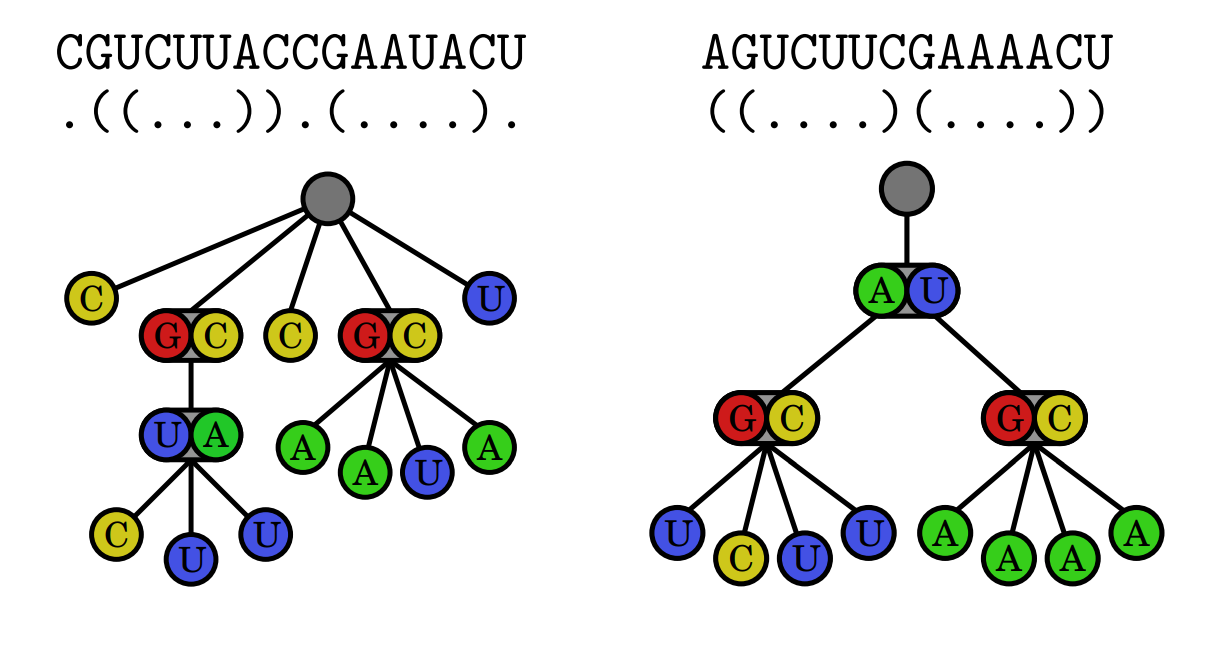
\includegraphics[width=\textwidth]{tree_sequences}}
    \end{overprint}
\end{frame}


\begin{frame}[c]{Tree-Alignment}
    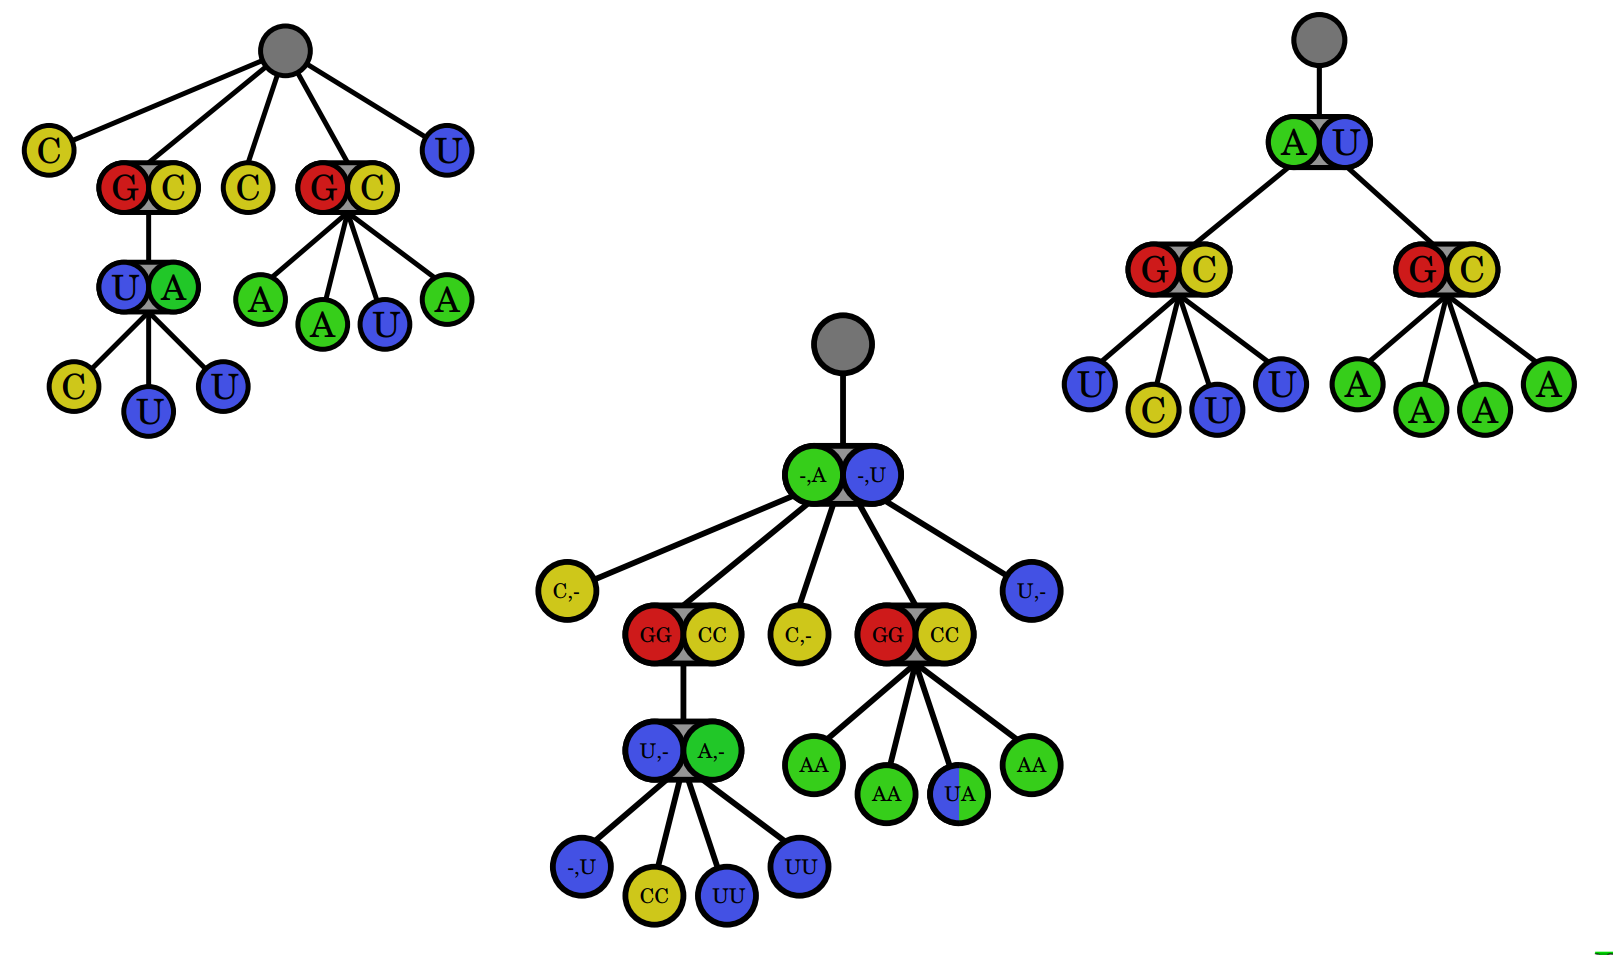
\includegraphics[width=1.03\textwidth]{tree_align}
\end{frame}

\begin{frame}[c]{Tree-Alignment Problems}
    \Large
    \begin{itemize}[<+(1)->]
        \item This is not always possible.
        \item There's structures that cannot be represented in trees.
        \newline
    \end{itemize}
    \pause
    Example: \texttt{(.[.).]}
\end{frame}



\begin{frame}[c]{Tree-Editing}
    \Large
    Edit operations on Trees ... \newline \pause
    ... are edit operations on arc-annotated sequences! \pause (\texttt{.((..(..)..))})
\end{frame}


\begin{frame}[c]{Tree-Editing Possibilities}
    % 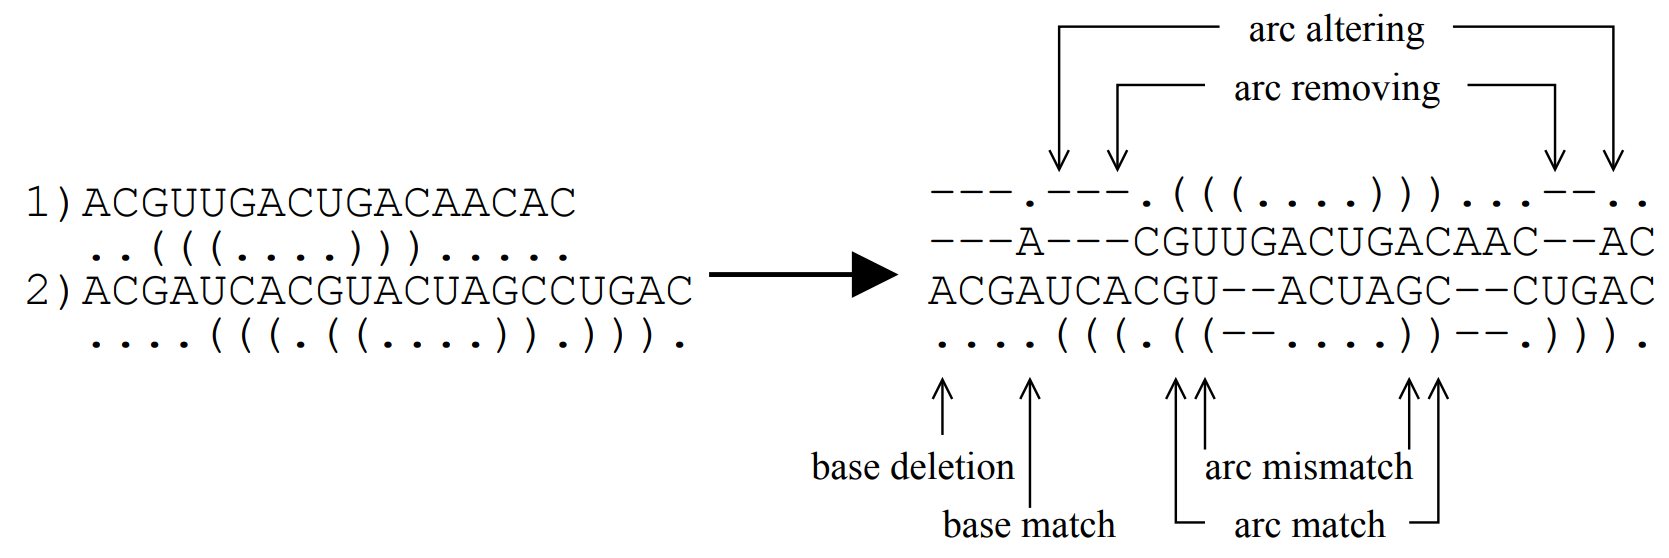
\includegraphics[width=\textwidth]{arc_things}
    \hspace{0mm}
    \begin{overprint}
    \onslide<1>\centering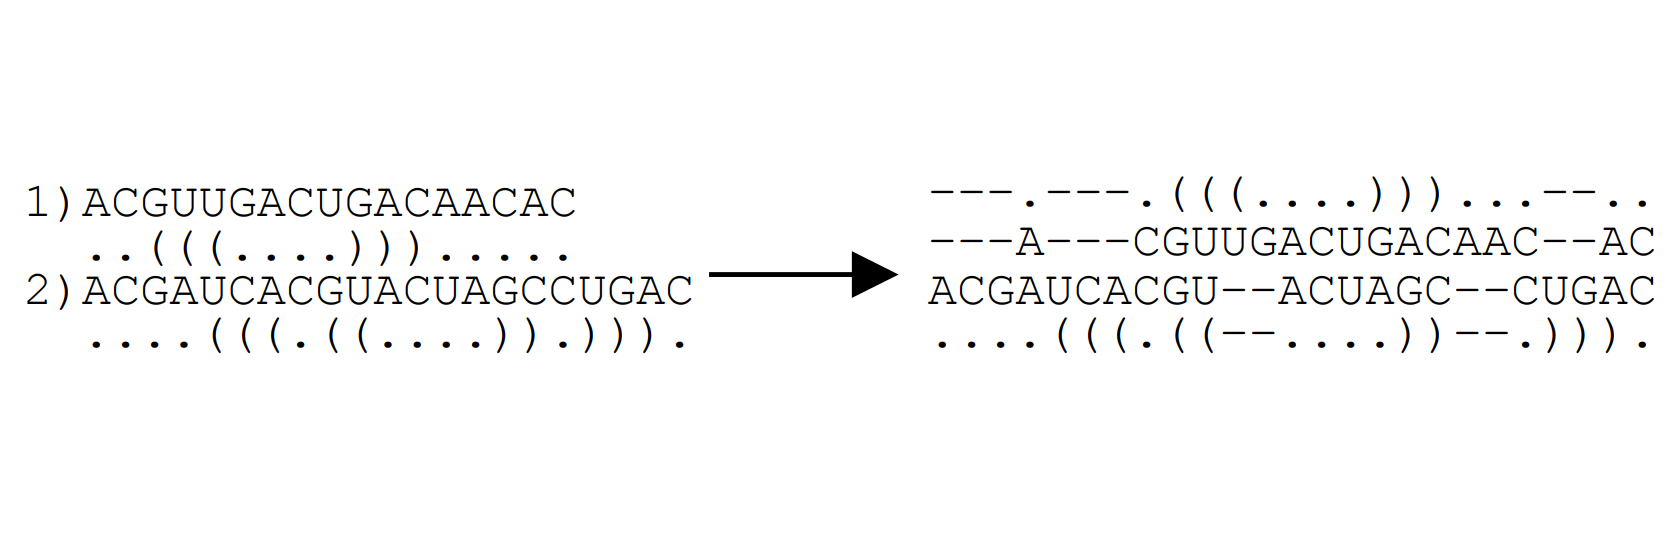
\includegraphics[width=\textwidth]{arc_example}
    \onslide<2>\centering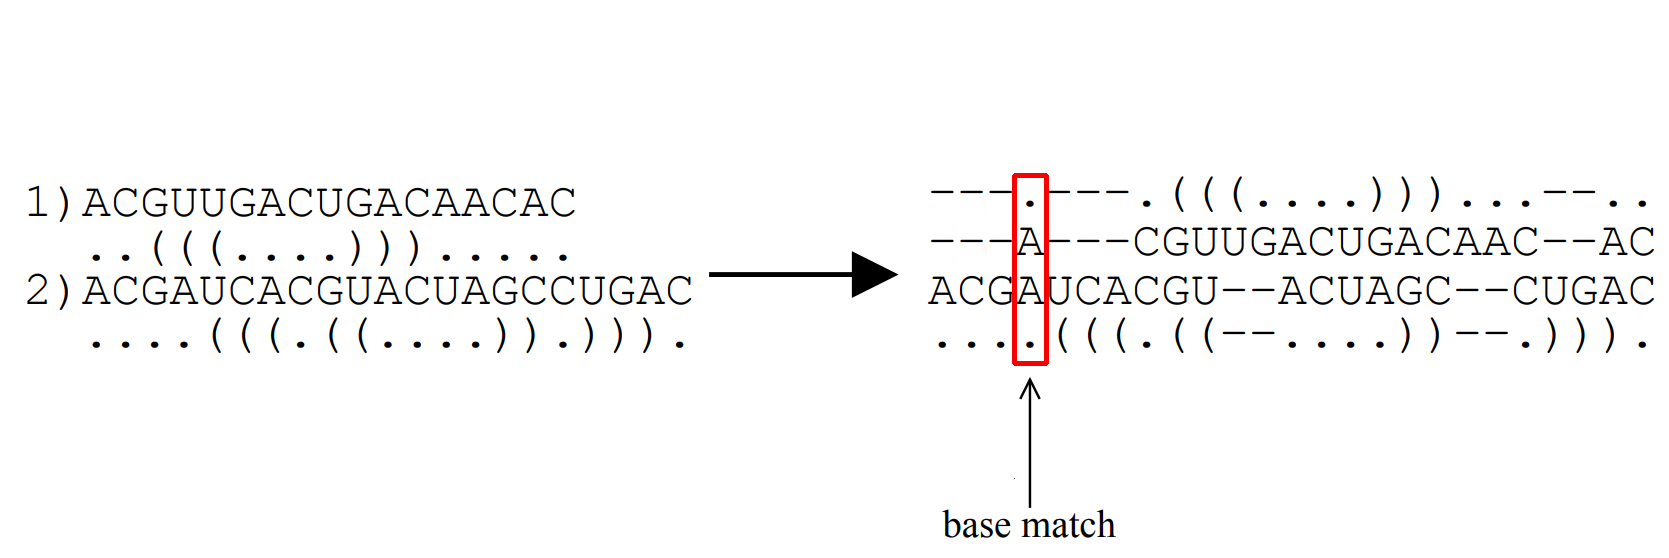
\includegraphics[width=\textwidth]{base_match}
    \onslide<3>\centering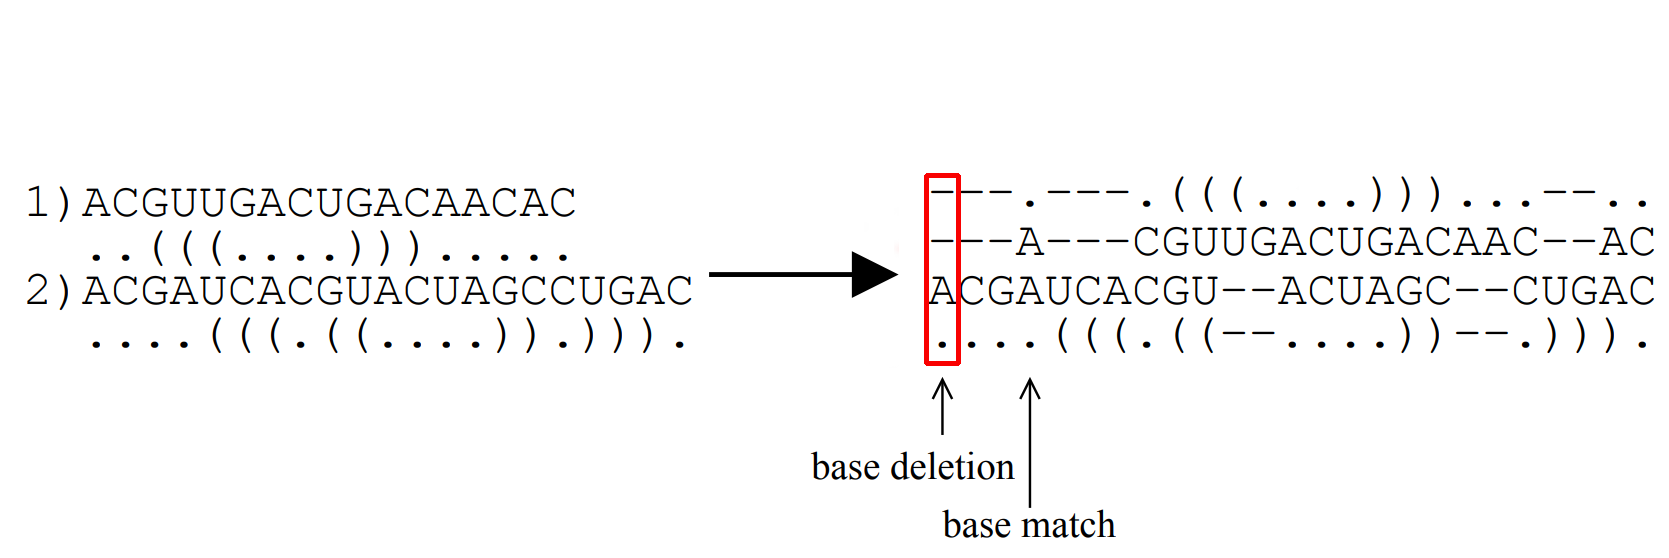
\includegraphics[width=\textwidth]{base_indel}
    \onslide<4>\centering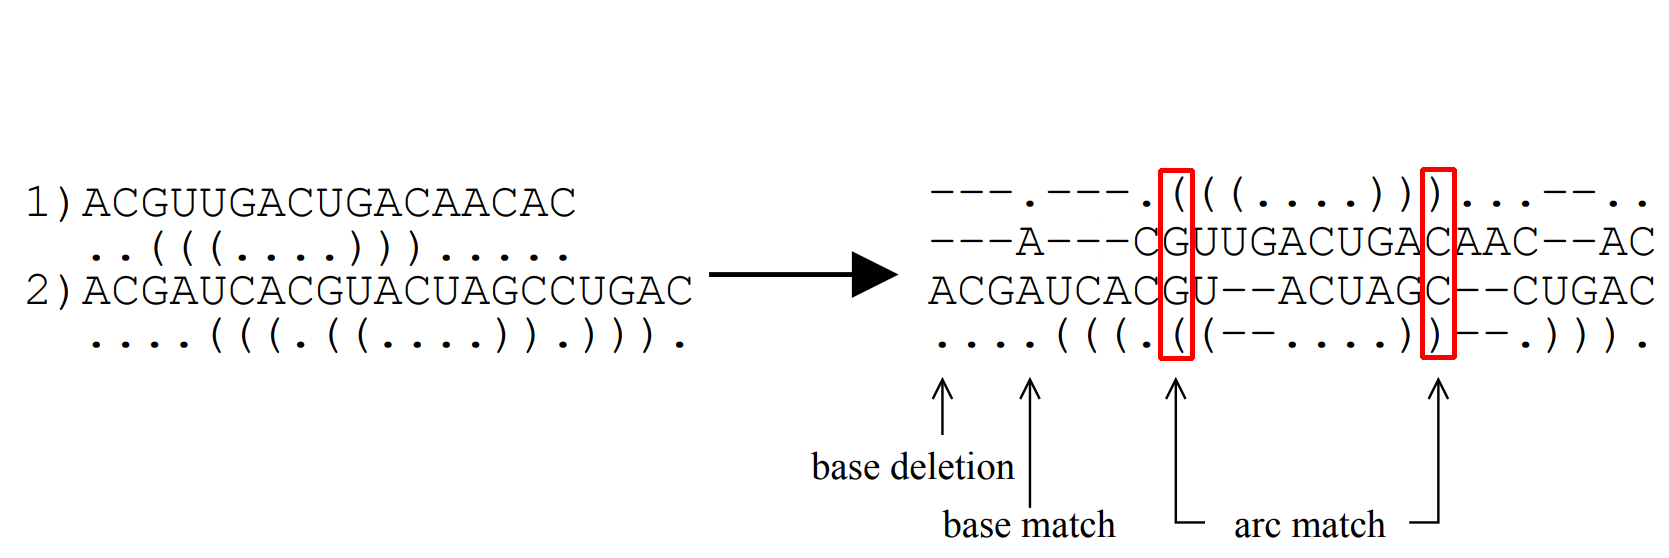
\includegraphics[width=\textwidth]{arc_match}
    \onslide<5>\centering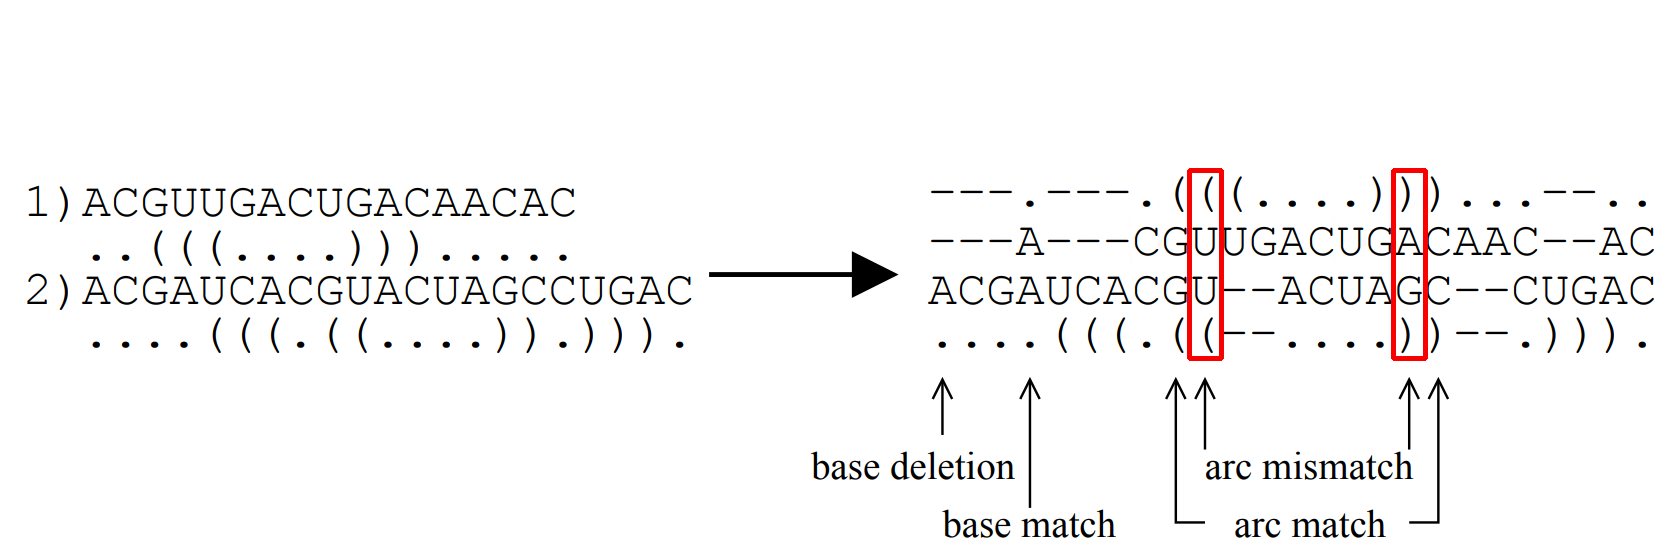
\includegraphics[width=\textwidth]{arc_mismatch}
    \onslide<6>\centering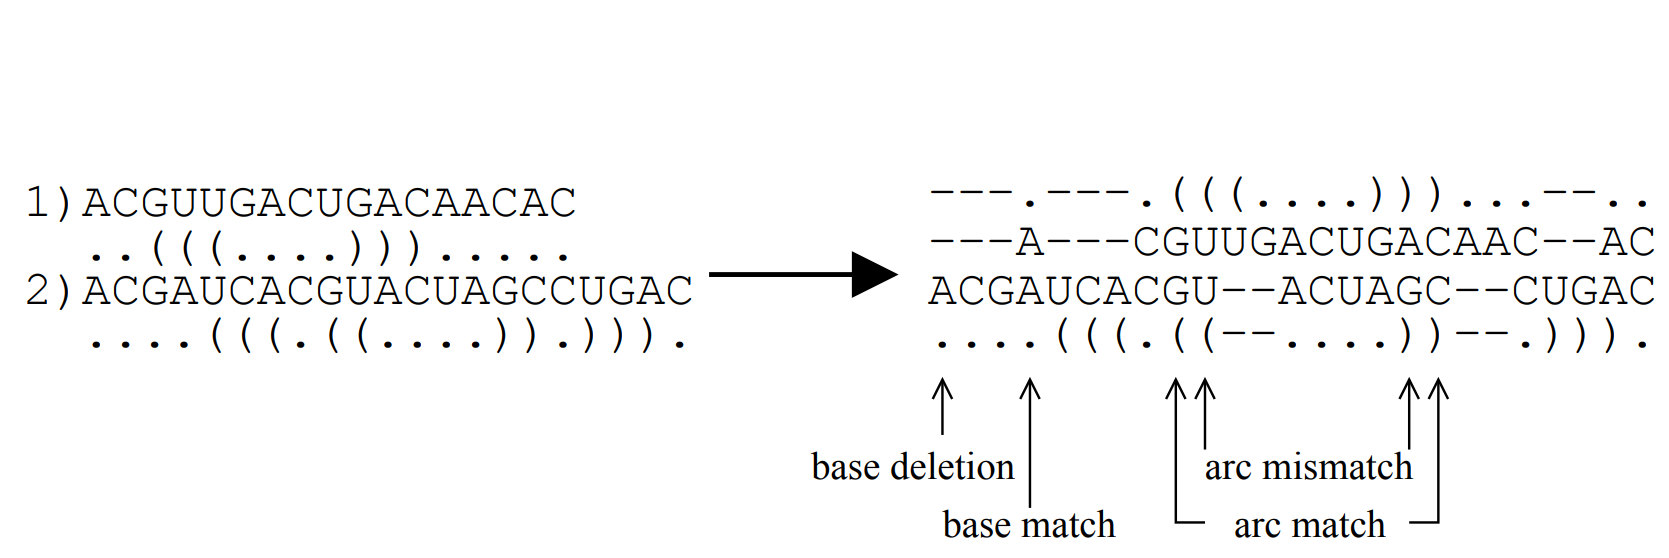
\includegraphics[width=\textwidth]{arc_breaking}
    \onslide<7>\centering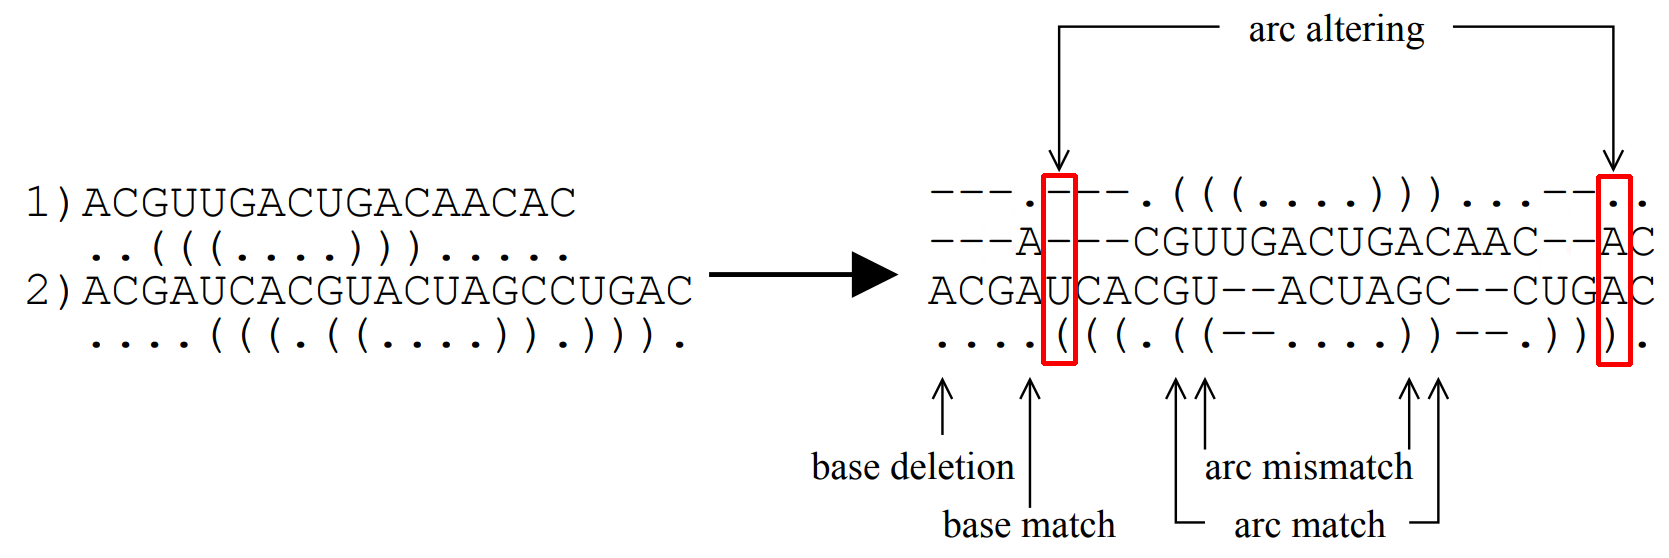
\includegraphics[width=\textwidth]{arc_altering}
    \onslide<8>\centering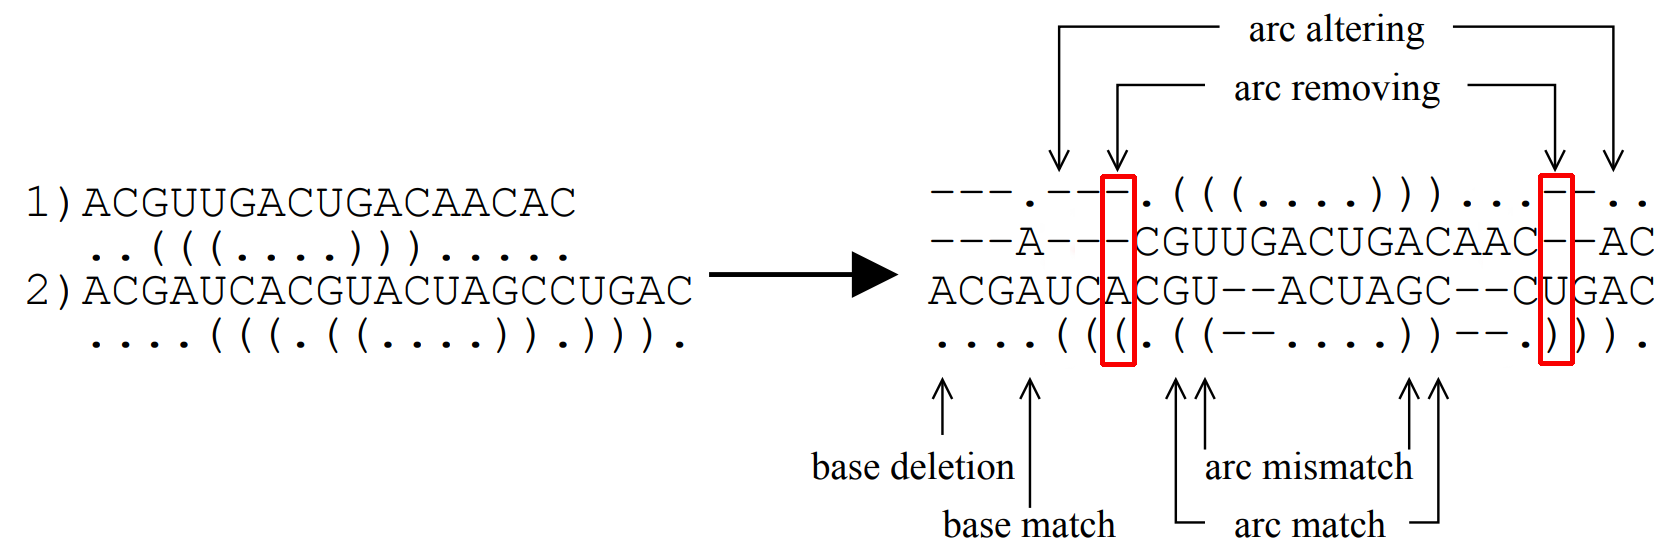
\includegraphics[width=\textwidth]{arc_removing}
    \end{overprint}

    \begin{multicols}{2}
    \begin{itemize}[<+(1)->]
        \item base match
        \item base indel
        \item arc match
            % arc on both strands match!
        \item arc mismatch
            % there is an arc on both, but there's different base pairs!
        \item arc breaking (missing)
            % there is an arc in one, but not in the other. Same bases though.
        \item arc altering
            % in one there's an arc, in the other only one of the two bases
        \item arc removing
            % there's nothing to resemble the arc in the other strand
    \end{itemize}
    \end{multicols}
\end{frame}

\begin{frame}[c]{Performance comparison}
    \hspace{0mm}
    \begin{overprint}
    \onslide<1>\centering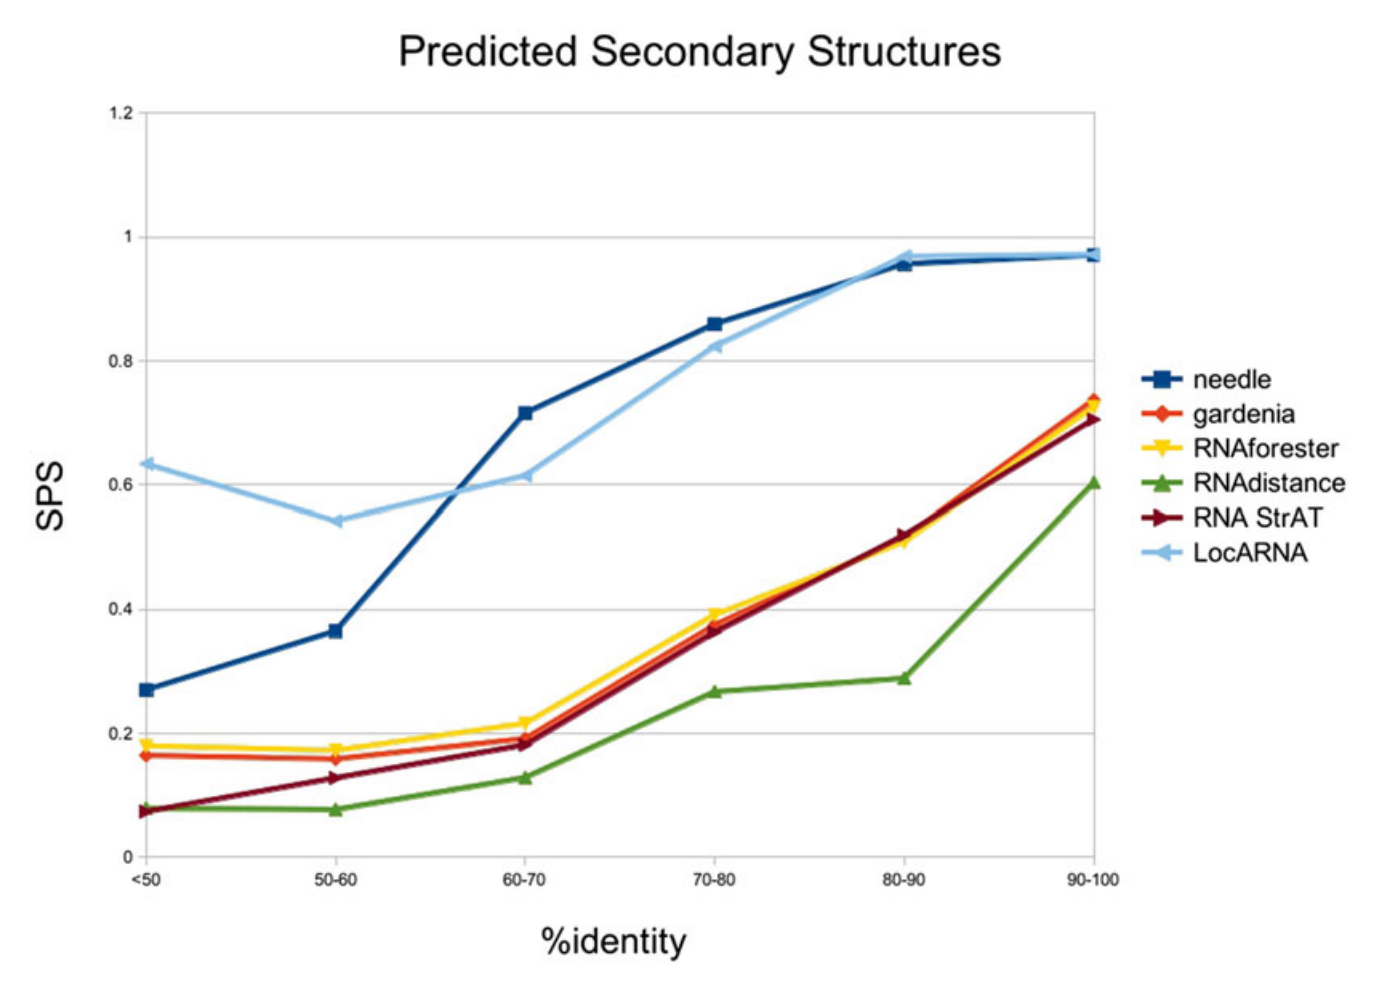
\includegraphics[width=0.9\textwidth]{predicted}
    \onslide<2>\centering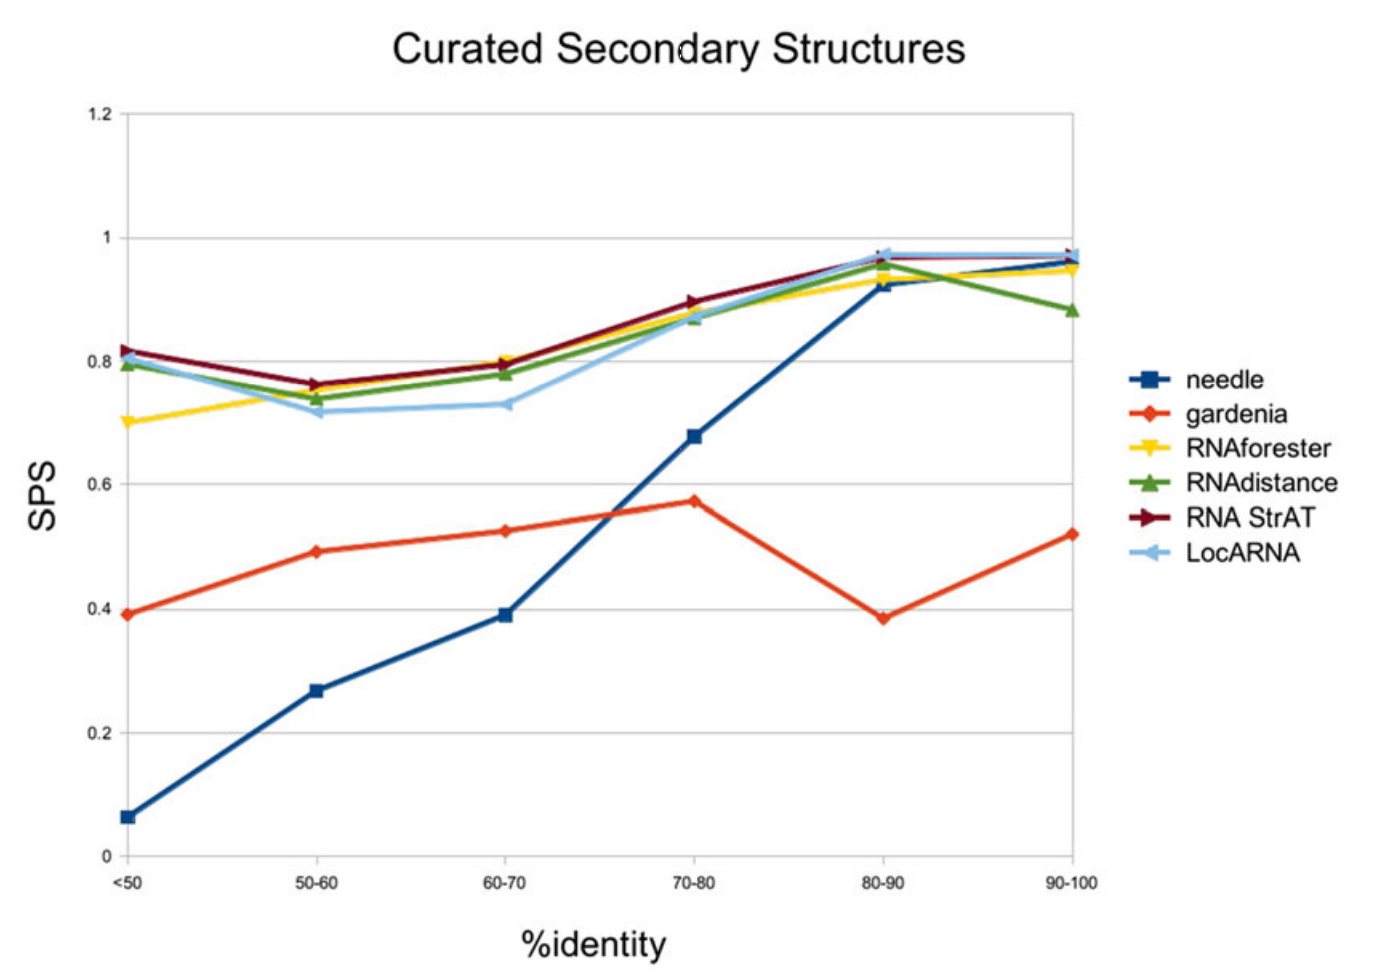
\includegraphics[width=0.9\textwidth]{curated}
    \end{overprint}
\end{frame}


\begin{frame}[c]{Tree-based Alignment}
    \Large
    \pause
    Basically a structure-using edit distance.
\end{frame}


% \section{Sankoff}


\begin{frame}[c]{Sankoff-Algorithm}
    \Large
    \begin{itemize}[<+(1)->]
    \item Dynamic Programming
    \item {\bf Space} needed: $O(n^4)$
    \item {\bf Runtime} $O(n^6)$
    \end{itemize}
    \pause
    What does it do ... ?
\end{frame}


\begin{frame}[c]{Sankoff-Algorithm}
    \Large
    Global free energy minimisation. \\
    \pause
    Considering every possible combination.
\end{frame}

% 
% \begin{frame}[c]{Sankoff-Algorithm}
%     \Large
%     \begin{itemize}[<+(1)->]
%     \item Base match
%     \item Base insertion
%     \item Base deletion
%     \item Base \textbf{pair} match
%     \end{itemize}
% \end{frame}






\section{LocARNA}

\begin{frame}[c]{LocARNA - Introduction}
    intro
\end{frame}



% \begin{frame}[c]{}
%     \Large
%     Cases:
%     \begin{itemize}[<+(1)->]
%     \item Base match
%     \item Base insertion
%     \item Base deletion
%     \item Base \textbf{pair} match
%     \end{itemize}
% \end{frame}



% 
\section{Sources}

%%%%%%%%%%%%%%%%%%%%%%%%%%CITES%%%%%%%%%%%%%%%%%%%%%%%%%%%%%
\begin{frame}[c,fragile,allowframebreaks]{Sources}
    The slides can be found at: \newline \newline

    \beamertemplatearticlebibitems
    \begin{thebibliography}{10}

    \bibitem{Github}
        {\bf Github}
        \newblock \url{https://github.com/fkarg/things-to-talk-about/tree/master/bioinfII}
    \newline

    \bibitem{Needleman-Wunsch Image}
            {\bf Needleman-Wunsch Image}
            \newblock \url{https://upload.wikimedia.org/wikipedia/commons/3/3f/Needleman-Wunsch_pairwise_sequence_alignment.png}

    \bibitem{Secondary structures Image}
            {\bf Secondary structures Image}
            \newblock \url{https://www.sciencedirect.com/science/article/pii/B9780124200371000014}

    \bibitem{RNA-Bioinformatics Lecture}
            {\bf RNA-Bioinformatics Lecture}
            \newblock \url{https://ilias.uni-freiburg.de/ilias.php?ref_id=1009368&obj\_id=1&cmd=layout&cmdClass=illmpresentationgui&cmdNode=fu&baseClass=ilLMPresentationGUI}


%     \beamertemplatebookbibitems
%     \bibitem{Richard Rumelt}
%         Richard Rumelt
%         \newblock {\em Good Strategy / Bad Strategy}.
%         \newblock The Difference and Why It Matters \\
%                   ISBN: 978-1-78125-154-6
%     \beamertemplatearticlebibitems
%     \bibitem{Lesswrong}
%         Lesswrong
%             \newblock {\em Expecting short Inferential Distances}
%             \newblock \url{http://lesswrong.com/lw/kg/expecting\_short\_inferential\_distances/}
%     \bibitem{Lesswrong}
%         Lesswrong
%             \newblock {\em Cached Thoughts}
%             \newblock \url{http://lesswrong.com/lw/k5/cached\_thoughts/}
%     \bibitem{Zenhabits}
%         Zenhabits
%             \newblock {\em say No so you can say YES}
%             \newblock \url{https://zenhabits.net/say-yes/}
%
%     \bibitem{Wikiquote}
%         Fukuzawa Yukichi
%             \newblock {\em Wikiquote}
%             \newblock \url{https://en.wikiquote.org/wiki/Fukuzawa\_Yukichi}
%
%     \bibitem{SpaceX}
%         SpaceX
%             \newblock {\em SpaceX}
%             \newblock \url{http://www.spacex.com/}
%
%    \bibitem{Wihipedia}
%        Wikipedia
%            \newblock {\em Proton-M}
%            \newblock \url{https://en.wikipedia.org/wiki/Proton-M}
%    \bibitem{Wikipedia}
%        Wikipedia
%            \newblock {\em Ariane 5}
%            \newblock \url{https://en.wikipedia.org/wiki/Ariane\_5}
%    \bibitem{Wikipedia}
%        Wikipedia
%            \newblock {\em Delta IV Heavy}
%            \newblock \url{https://en.wikipedia.org/wiki/Delta\_IV}
   \end{thebibliography}
    % required the allowframebreaks for longer lists

\end{frame}







%%%%%%%%%%%%%%%%%%%%%%%%%%%%%%%%%%%%%%%%%%%%%%%%%%%%%%%%%%%%%%%%%%%%%%%%%%%%%%%%%%%%%%%%%%%%%%%%%%%%%%%%%%%%%%%%%%%


\end{document}
